%% Los cap'itulos inician con \chapter{T'itulo}, estos aparecen numerados y
%% se incluyen en el 'indice general.
%%
%% Recuerda que aqu'i ya puedes escribir acentos como: 'a, 'e, 'i, etc.
%% La letra n con tilde es: 'n.
\chapter{Pruebas de Funcionalidad}
En este cap\'itulo se realizan un conjunto de pruebas de correctitud y optimizaci\'on para demostrar el buen funcionamiento de las herramientas implementadas y as\'i evidenciar el cumplimiento de los objetivos planteados en el trabajo.

Las pruebas se realizaron en una laptop con las siguientes caracter\'isticas:
\begin{itemize}
\item Sistema operativo Windows 10 Enterprise LTSC, 64 bits.
\item Procesador Intel(R) Core(TM) i3-6100U @ 2.30GHz 2.30GHz.
\item Memoria RAM: 8GB (7.82 usable)
\item Disco duro 250GB, HDD.
\end{itemize}

Se cuenta con la cartograf\'ia de GeoCuba para las pruebas, las cuales iniciaron con los siguentes datos guardados en la base de datos de Admin: 
\begin{itemize}
\item Capa \textbf{Roads}(Calles), color rojo definido por defecto, con informaci\'on alfanum\'erica asociada de cinco columnas: \textit{maxspeed}, \textit{oneway}, \textit{bridge}, \textit{type}, \textit{name}.
\item Un usuario con rol de Administrador, \textit{adminopenlatino@gmail.com}.
\item Workspace \textit{AdminWorkspace}, asociado al usuario anterior, con acceso a las funciones \textit{GetCapabilities}, \textit{GetMap} y \textit{GetTematicMap}.
\item Estilos \textit{RedStyle}, \textit{BlueStyle}, \textit{GreenStyle} y \textit{YellowStyle} que representan los colores, rojo, azul, verde y amarillo respectivamente.
\end{itemize}

Para la validaci\'on de las pruebas se usar\'a Postman, verificando mediante este que el sistema est\'a funcionando correctamente. Postman es una aplicaci\'on que permite realizar pruebas API. Es un cliente HTTP\footnote{HTTP, de sus siglas en ingl\'es: Hypertext Transfer Protocol, es el nombre de un protocolo que permite realizar una petici\'on de datos y recursos.} que da la posibilidad de realizar \textit{HTTP requests} a trav\'es de una interfaz gr\'afica de usuario, por medio de la cual se obtiene la respuesta del servidor.

\section{Configuraci\'on de tem\'aticos por categor\'ias}
El objetivo de esta prueba es crear un nuevo tem\'atico en OLS. Se trabajar\'a sobre la capa \textbf{Roads}, escogiendo la columna \textit{oneway}\footnote{Seg\'un la cartograf\'ia de GeoCuba, este campo tiene valor 1 si la calle es de un solo sentido y 0 en caso contrario} como campo alfanum\'erico. La figura \ref{create} muestra la vista de creaci\'on con los datos anteriores.

\begin{figure}[h]
\centering
\label{create}
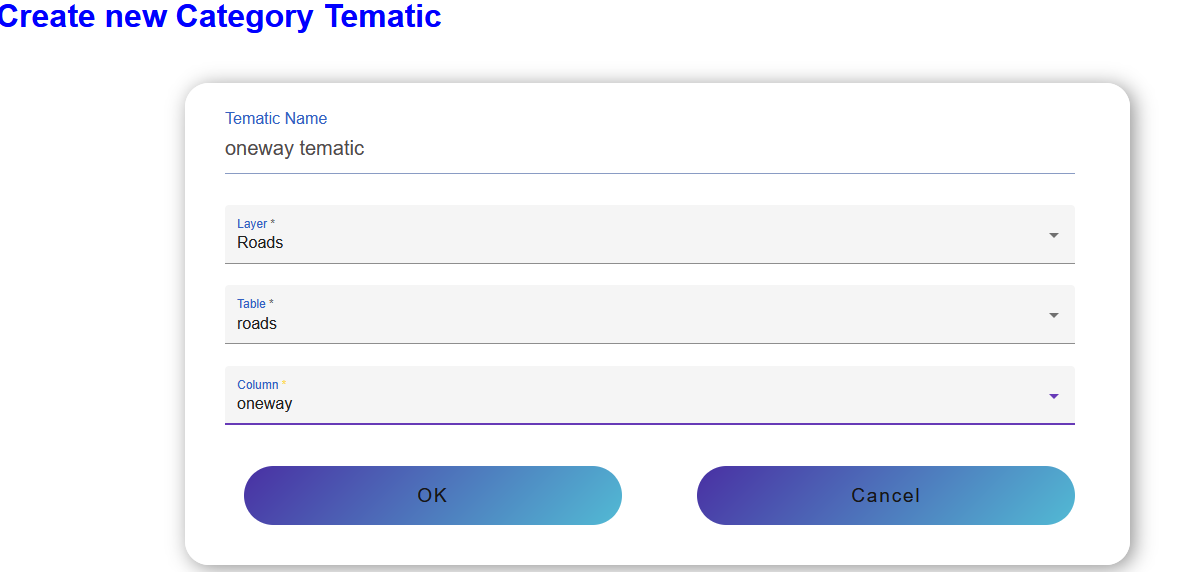
\includegraphics[scale=0.5]{images/createTematic.png} 
\caption{Vista de creaci\'on de tem\'aticos de categor\'ias.}
\end{figure}

Se espera que se genere una configuraci\'on de tem\'atico donde se tienen dos estilos para dos categor\'ias. Efectivamente, se comprueba que dando click en el bot\'on \textbf{OK}, se genera la configuraci\'on del tem\'atico autom\'aticamente, observ\'andose en la figura \ref{config} las dos posibles categor\'ias de la columna seleccionada, y la asignaci\'on de estilos. Si no hay suficientes estilos para cada categor\'ia el usuario puede generarlos desde esta vista. El usuario tambi\'en tiene la posibilidad de cambiar los estilos asignados por otros o crear uno nuevo.

\begin{figure}[h]
\centering
\label{config}
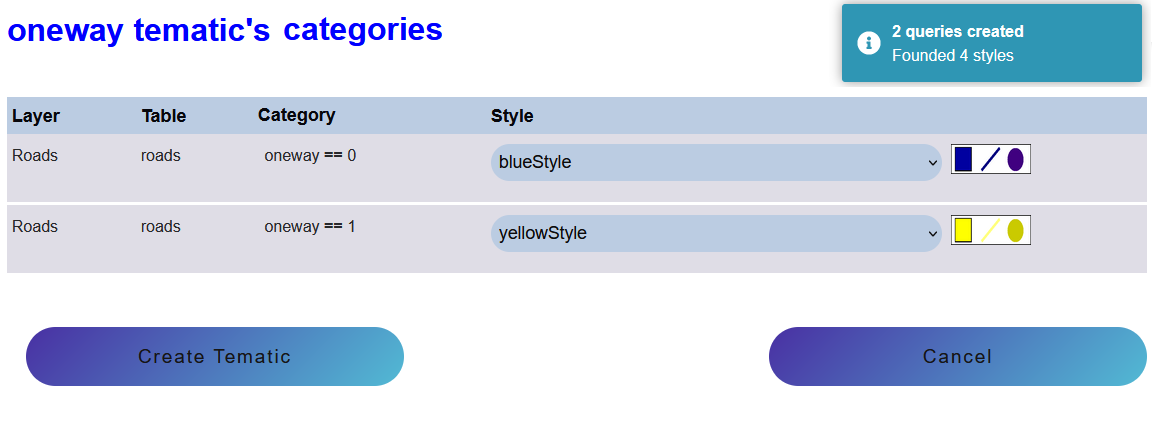
\includegraphics[scale=0.4]{images/configTematic.png}
\caption{Configuraci\'on generada a partir de los datos de la vista de creaci\'on.}
\end{figure}

Si se da click sobre el bot\'on \textbf{Create Tematic}, se genera el nuevo tem\'atico como se observa en la figura \ref{listTematic}. La cual muestra una lista de todos los tem\'aticos de ese tipo creados, en este caso, solo existe el tem\'atico de nombre \textit{oneway tematic}. Adem\'as, se observa la informaci\'on asociada a este: capa, categor\'ias, estilos, etc.

\begin{figure}[h]
\centering
\label{listTematic}
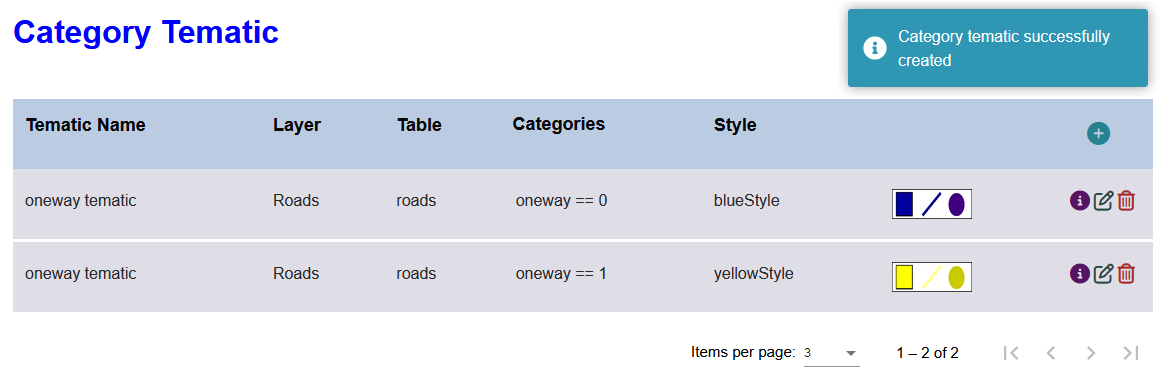
\includegraphics[scale=0.4]{images/listTematic.png} 
\caption{Listado de mapas tem\'aticos creados en OLS.}
\end{figure}


\section{Generaci\'on de mapas tem\'aticos por categor\'ias.}
Mediante postman se verifica que el tem\'atico creado en la secci\'on anterior se pinta bien sobre el mapa. Se espera que al realizar el pedido, se coloreen las calles de un solo sentido de azul y las de dos sentidos de amarillo. Si existe alguna calle que no tenga definido sentido en la cartograf\'ia, debido a que este valor es NULL, se pinta del valor por defecto de las calles, en este caso, rojo.

\begin{figure}[h]
\centering
\label{postmanTematic}
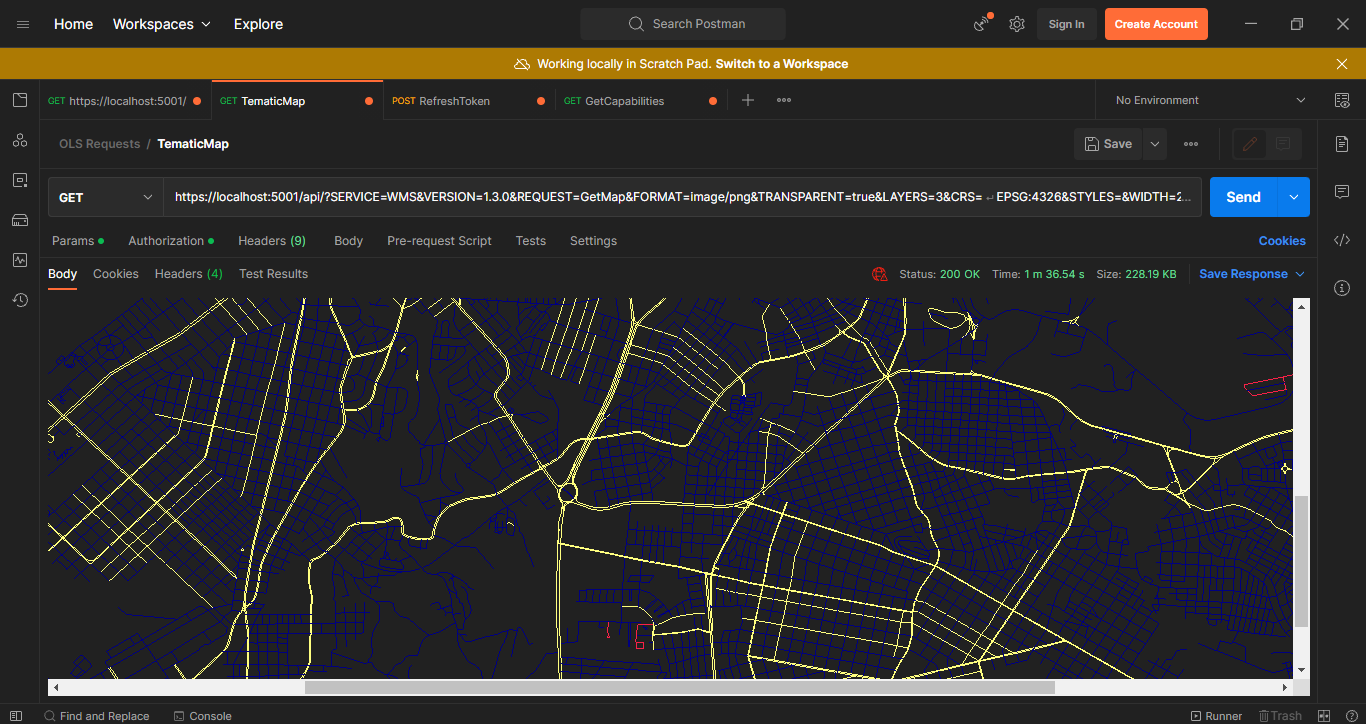
\includegraphics[scale=0.4]{images/postmanTematic.png} 
\caption{Pedido \textit{GetTematicMap.}}
\end{figure}

La figura \ref{postmanTematic} muestra la respuesta del servidor para el tem\'atico reci\'en creado. Se observan los resultados esperados. Ahora se edita el tem\'atico, para en lugar de pintar las calles de amarillo, lo haga de verde (figura \ref{editTematic}).

\begin{figure}[h]
\centering
\label{editTematic}
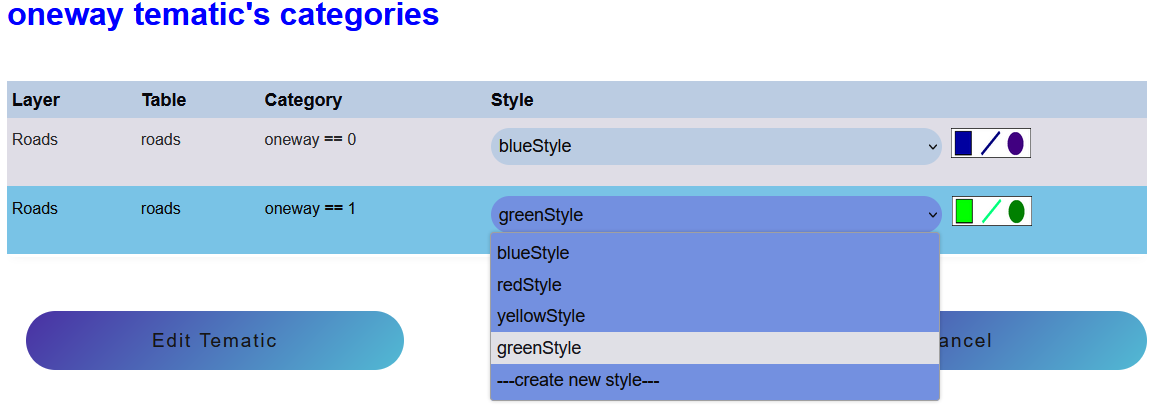
\includegraphics[scale=0.4]{images/editTematic.png} 
\caption{Edici\'on de tem\'aticos.}
\end{figure}

Si se realiza nuevamente el pedido se observa que ahora las calles de doble sentido est\'an coloreadas de verde.(figura \ref{postman2})

\begin{figure}[h]
\centering
\label{postman2}
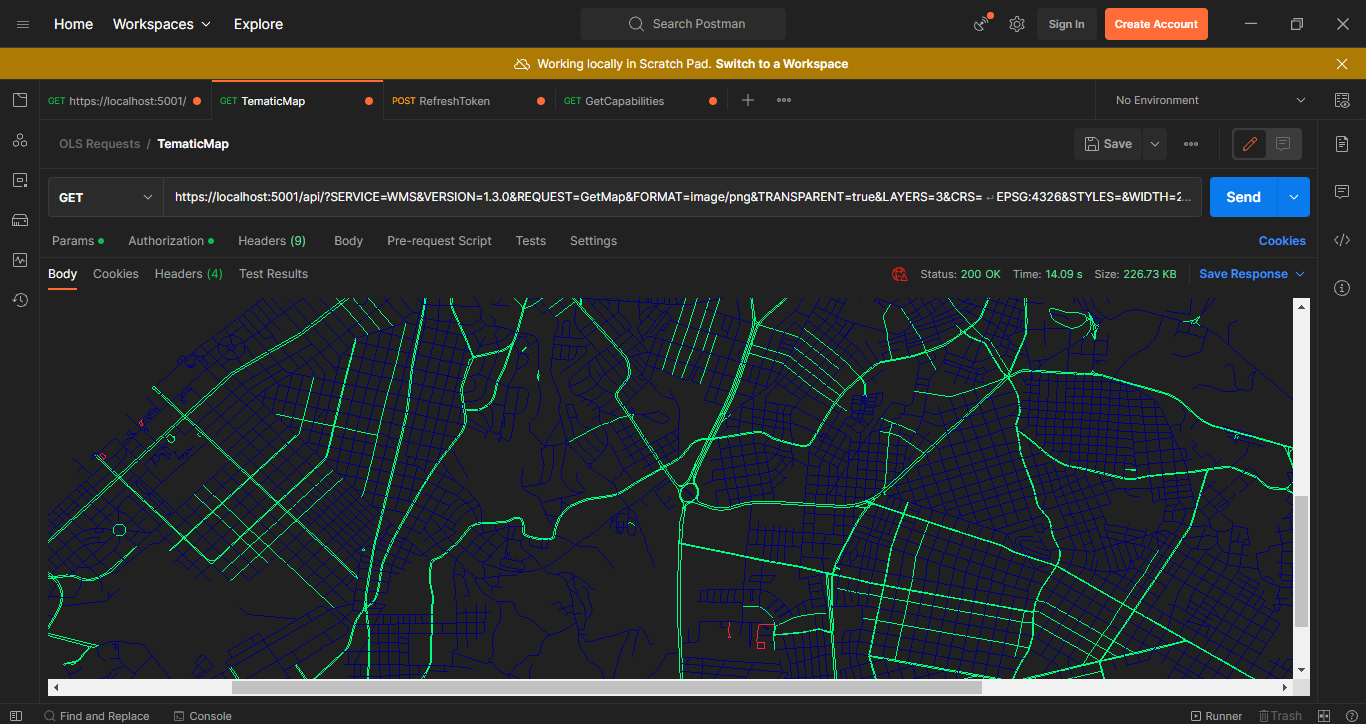
\includegraphics[scale=0.4]{images/postmanTematic2.png} 
\caption{Pedido \textit{GetTematicMap} a tem\'atico editado.}
\vspace{5cm}
\end{figure}



\section{Comprobaciones a la interfaz visual}
En esta prueba se verifica que la interfaz visual est\'a funcinando correctamente mediante operaciones CRUD. Para ello se trabaja con la entidad \textit{estilos}, y funciona de manera an\'aloga para el resto de las entidades. Primeramente, el estilo de color verde, se editar\'a y pasar\'a a ser de color celeste, elimin\'andolo finalmente del servidor.

La figura \ref{estilo} muestra la vista de edici\'on, y los listados de estilo despu\'es de editado. Se observan los resultados esperados. Finalmente, se eliminar\'a este estilo del sistema. La figura \ref{deleteStyle} muestra que esta operaci\'on se realiz\'o satisfactoriamente.

\begin{figure}[h]
\centering
\label{estilo}
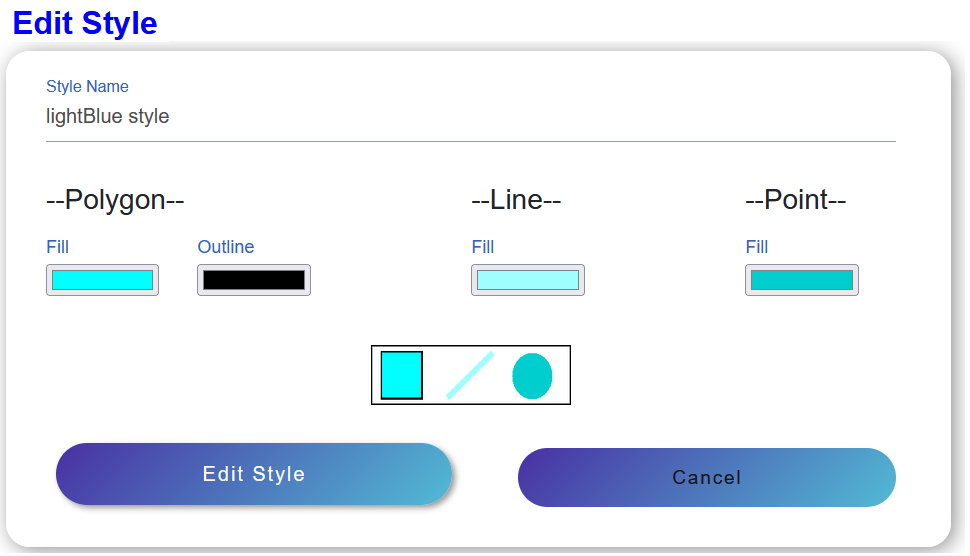
\includegraphics[scale=0.3]{images/editStyle.png} 
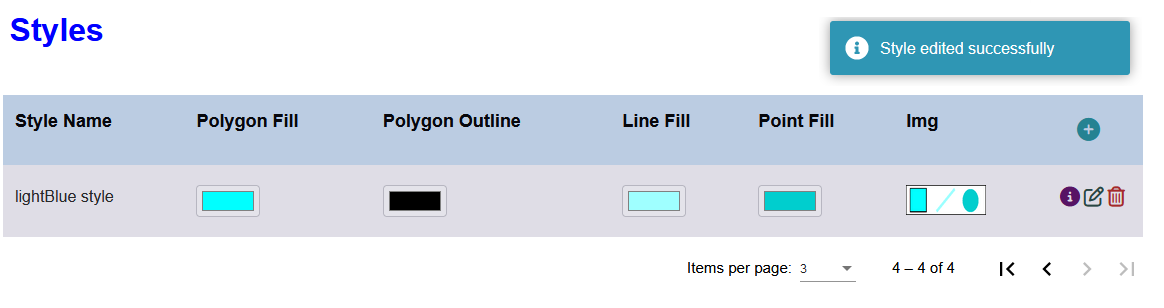
\includegraphics[scale=0.3]{images/listStyle.png} 
\caption{Edici\'on de estilos.}
\end{figure}

\begin{figure}[h]
\centering
\label{deleteStyle} 
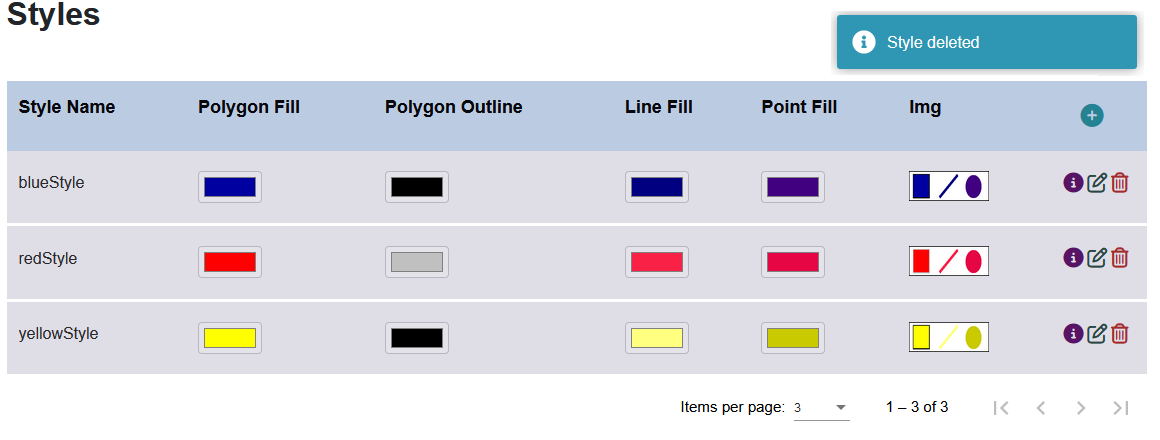
\includegraphics[scale=0.3]{images/deleteStyle.png} 
\caption{Eliminaci\'on de estilos.}
\end{figure}






%-------------------------------------------------------------------------------------------------------------------------------------
%-------------------------------------------------------------------------------------------------------------------------------------

\chapter{Conclusiones, recomendaciones y trabajo futuro}
La implementaci\'on de las funcionalidades expuestas en cap\'itulos anteriores da soluci\'on a las deficiencias planteadas de OLS, por lo tanto, se cumplieron los objetivos propuestos. 

En este cap\'itulo se exponen las conclusiones a las que se arribaron con el desarrollo de la aplicaci\'on y se proponen, adem\'as, algunas recomendaciones para el trabajo futuro con OLS.

\section{Conclusiones}
El presente trabajo de diploma finaliza con la creaci\'on de la nueva interfaz visual de OLS, intuitiva, agradable y segura. Para lograrlo, se realizaron modificaciones sobre el sistema, en su arquitectura, modelo de datos y desarrollo de nuevas funcionalidades, con una implementaci\'on extensible y reusable, manteniendo las buenas pr\'acticas que presenta el servidor. Se cre\'o, adem\'as, un nuevo tipo de tem\'atico, por clasificaci\'on de tipos o por categor\'ias, que le permite al usuario la creaci\'on de mapas tem\'aticos de forma sencilla, ya que todo el procesamiento de los datos y asignaci\'on de estilos se realiza de forma autom\'atica,  extendiendo, para lograr este prop\'osito, el \textit{Render}(clase encargada de pintar los mapas) de OLS, para que aceptara filtros gen\'ericos, en lugar de consultas sql. Por \'ultimo, se modific\'o el pedido \textit{GetCapabilities} para que este muestre tambi\'en la informaci\'on acerca de los tem\'aticos existentes, tambi\'en se cre\'o un nuevo pedido \textit{GetTematicCapabilities}, que devuelve solo la informaci\'on de los mapas tem\'aticos creados.

Estos cambios mencionados dotan a OLS de mejoras y nuevas funcionalidades, por lo que se puede concluir que los principales aportes de esta investigaci\'on son:

\begin{itemize}
\item Modificaci\'on del pedido \textit{GetCapabilities} para que devuelva informaci\'on acerca de mapas tem\'aticos y creaci\'on de un nuevo pedido que devuelve solo esa informaci\'on.
\item Implementaci\'on de una nueva interfaz visual, mediante la cual se puede modificar la configuraci\'on de OLS de forma intuitiva.
\item Creaci\'on de un nuevo tipo de mapa tem\'atico que realiza el procesamiento de capas, categor\'ias asociadas y estilos autom\'aticamente.
\item Modificaci\'on de la arquitectura de OLS para acoplar la nueva interfaz visual, implementada en Angular, y la seguridad de los pedidos de los usuarios.
\item Cambio del modelo de datos para la implementaci\'on del nuevo tem\'atico y hacer extensible el proceso de agregar nuevos tipos.
\item Nueva implementaci\'on del Render para que acepte filtros gen\'ericos (varias condiciones separadas por operadores l\'ogicos) en lugar de consultas sql.
\end{itemize}


\section{Recomendaciones y trabajo futuro}
Aunque se cumpli\'o con todos los objetivos planteados al inicio del trabajo, el software implementado puede mejorarse y se pueden agregar nuevas funcionalidades, por ello, se propone:

\begin{itemize}
\item Mejorar la arquitectura usada en la interfaz visual. Para su desarrollo se us\'o la arquitectura propia del framework, sin embargo, puede implementarse arquitectura de capas y patr\'on MVC.
\item Implementar nuevos tipos de tem\'aticos que refuercen las funcionalidades de OLS como servidor de mapas.
\item Mejorar la implementaci\'on de los controladores, con el objetivo de refactorizar c\'odigo y mantener las buenas pr\'acticas de la programaci\'on.
\item Migrar el servidor OLS a la \'ultima versi\'on de .NET Core.
\end{itemize}